\documentclass[12pt, reqno]{article}
\usepackage{enumerate,amsmath,amssymb,bm,ascmac,amsthm,url}
\usepackage{tikz}
\usetikzlibrary{calc}

\begin{document}

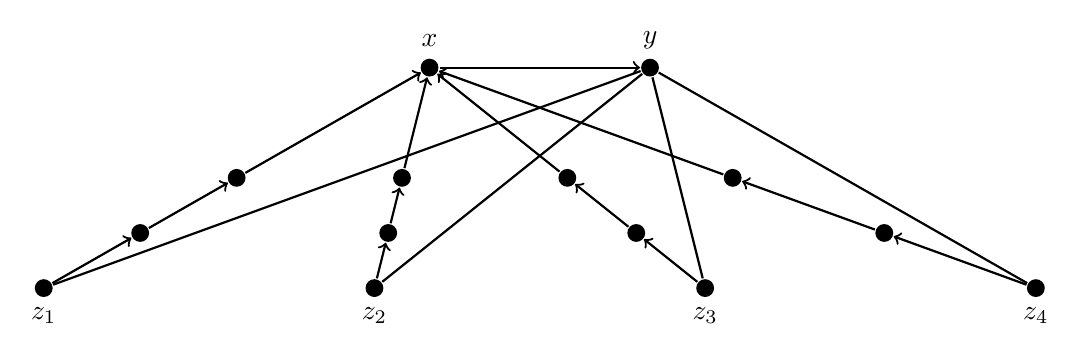
\begin{tikzpicture}
[scale = 0.7,
line width = 0.8pt,
v/.style = {circle, fill = black, inner sep = 0.8mm},u/.style = {circle, fill = white, inner sep = 0.1mm}]
\node[u] (Lx) at (-2, 0.5) {$x$};
\node[u] (Ly) at (2, 0.5) {$y$};
\node[u] (Lz1) at (-9, -4.5) {$z_1$};
\node[u] (Lz2) at (-3, -4.5) {$z_2$};
\node[u] (Lz3) at (3, -4.5) {$z_3$};
\node[u] (Lz4) at (9, -4.5) {$z_4$};
%
\node[v] (x) at (-2, 0) {};
\node[v] (y) at (2, 0) {};
%
\node[v] (z1) at (-9, -4) {};
\node[v] (z1x) at (-5.5, -2) {};
\node[v] (z1x2) at (-7.25, -3) {};
%
\node[v] (z2) at (-3, -4) {};
\node[v] (z2x) at (-2.5, -2) {};
\node[v] (z2x2) at (-2.75, -3) {};
%
\node[v] (z3) at (3, -4) {};
\node[v] (z3x) at (0.5, -2) {};
\node[v] (z3x2) at (1.75, -3) {};
%
\node[v] (z4) at (9, -4) {};  
\node[v] (z4x) at (3.5, -2) {};
\node[v] (z4x2) at (6.25, -3) {};
%
\draw[->] (x) to (y);
%
\draw[->] (z1) to (z1x2);
\draw[->] (z1x2) to (z1x);
\draw[->] (z1x) to (x);
\draw[-] (y) to (z1);
%
\draw[->] (z2) to (z2x2);
\draw[->] (z2x2) to (z2x);
\draw[->] (z2x) to (x);
\draw[-] (y) to (z2);
%
\draw[->] (z3) to (z3x2);
\draw[->] (z3x2) to (z3x);
\draw[->] (z3x) to (x);
\draw[-] (y) to (z3);
%
\draw[->] (z4) to (z4x2);
\draw[->] (z4x2) to (z4x);
\draw[->] (z4x) to (x);
\draw[-] (y) to (z4);
\end{tikzpicture}

\end{document}